%!TEX root = ../main.tex

\section{Conditional Diversification Benefit} % (fold)
\label{sec:conditional_diversification_benefit}

This section studies a new measure of diversification in a portfolio called \emph{conditional diversification benefit} (CDB), which is developed by \textcite{ChristoffersenErrunzaJacobLanglois2012}. CDB is based on the portfolio expected shortfall (ES), i.e. the expected loss in case the return materializes below a certain percentile, and therefore concerns the properties of the tail of the portfolio distribution. As already described, if factors are not multivariate normal, the covariance matrix used in mean-variance optimization is not a full description of the dependency between factors. Factor returns are not normal, and therefore higher moments influence the tail behavior of their returns. These considerations are important for any portfolio looking to manage risk by diversifying across factors.
For a portfolio manager looking to manage risk by diversifying across factors, such considerations are important

In this section, all distributions of portfolio returns are simulated from our Student's \textit{t} dynamic copula model.

We begin by describing the construction and intuition of CDB and subsequently present the CDB over time for different five- and six-factor asset universes, including and excluding HML and CMA.

\subsection{Formula and interpretation of the CDB statistic}

Define ES as the expected loss in some bottom percentile $q$
\begin{align}
    \text{ES}_{i,t}^q(r_{i,t}) = -\mathbb{E}[r_{i,t} | r_{i,t} \leq F_{i,t}^{-1}(q)]
\end{align}
where $F_{i,t}^{-1}(q)$ is the inverse CDF of simple returns $r_{i,t}$ at $q$ (equivalent to the $q\%$ Value-at-Risk). 

The expected shortfall represents the expected loss when returns realize below the Value-at-Risk of the portfolio. Depending on the distribution at hand, the expected shortfall can be closer or further to the Value-at-Risk. Intuitively, if assets offer little diversification, then no combination of assets will reduce total portfolio risk; and ES will be high. 

For a portfolio of assets with weights $w_t$, the portfolio's ES as a function of weights: $\text{ES}_t^q(w_t)$, has an upper bound equal to the weighted average of each asset's ES, corresponding to the case of no diversification~\autocite{Artzner1999}:
\begin{align}
  \overline{\text{ES}}_t^q(w_t) = \sum_{i=1}^N w_{i,t} \text{ES}_{i,t}^q(r_{i,t})
\end{align}
A lower bound on portfolio ES is instead given by the portfolio's Value-at-Risk ($-F_{t}^{-1}(w_t, q)$), which corresponds to the case of perfect diversification:
\begin{align}
  \underline{\text{ES}}_t^q(w_t) = -F_{t}^{-1}(w_t, q)
\end{align}
CDB is defined as the portfolio's ES scaled by its lower and upper bounds:
\begin{align}
  \text{CDB}_t^q(w_t) = \frac{\overline{\text{ES}}_t^q(w_t) - \text{ES}_t^q(w_t)}{\overline{\text{ES}}_t^q(w_t) - \underline{\text{ES}}_t^q(w_t)}
\end{align}
The intuition behind the statistic is best understood by focusing on the second term of the numerator and the denominator: when diversification benefits are high, the expected shortfall of a portfolio $\text{ES}_t^q(w_t)$ in the numerator is relatively close to the Value-at-Risk, i.e. the lower bound: $\underline{\text{ES}}_t^q(w_t)$ in the denominator, which makes the ratio close to one. 

Focusing instead on the numerator only: when diversification benefits are low, the expected shortfall $\text{ES}_t^q(w_t)$ is hardly different from its upper bound: $\overline{\text{ES}}_t^q(w_t)$, and the ratio is close to zero.

In summary, CDB is a number between zero and one where one represents perfect diversification, and zero no diversification. CDB is a measure of diversification only -- the level of expected return across factors does not enter the equation.

A closed formula for CDB of a portfolio does not exist if returns are not normal. We use the same simulated returns as in the previous section to form the return distribution of factors each week, and combine them into portfolios subject to the same conditions as for the mean-variance exercise (all weights sum to one; all weights positive). We then run a maximization algorithm for CDB, finding the combination of weights that give the highest possible diversification:
\begin{align*}
  \arg\!\max_{w_t} \text{CDB}_t^q(w_t)
    && \text{s.t.} \sum_{i=1}^N w_{i,t} = 1 \\
    && w_{i,t} \ge 0 \,\, \forall i
\end{align*}

The ES is based on the simulated return distributions in each period, as modeled by the dynamic Student's \textit{t} copula. We present results based on a Value-at-Risk cut-off of 5\% -- results based on lower values (e.g. 1\%) are qualitatively similar.

\subsection{CDB results for different asset universes}
% Picture different between 5-factor and 6-factor
\autoref{fig:cdb} plots conditional diversification benefit measures of the five- and six-factor asset universes, including and excluding HML and CMA. We have smoothed the plots using quarterly moving averages in order to make them easier to read. We proceed with a number of interesting results that emerge from this picture:

\begin{figure}
  \centering
  \footnotesize
  \renewcommand{\arraystretch}{1.2}
  \caption{5\% Conditional diversification benefit (CDB) for six different asset universes, full sample (1963--2016). 
  The line has been smoothed with a moving average on a quarterly window to make it easier to read.}
  \label{fig:cdb}
  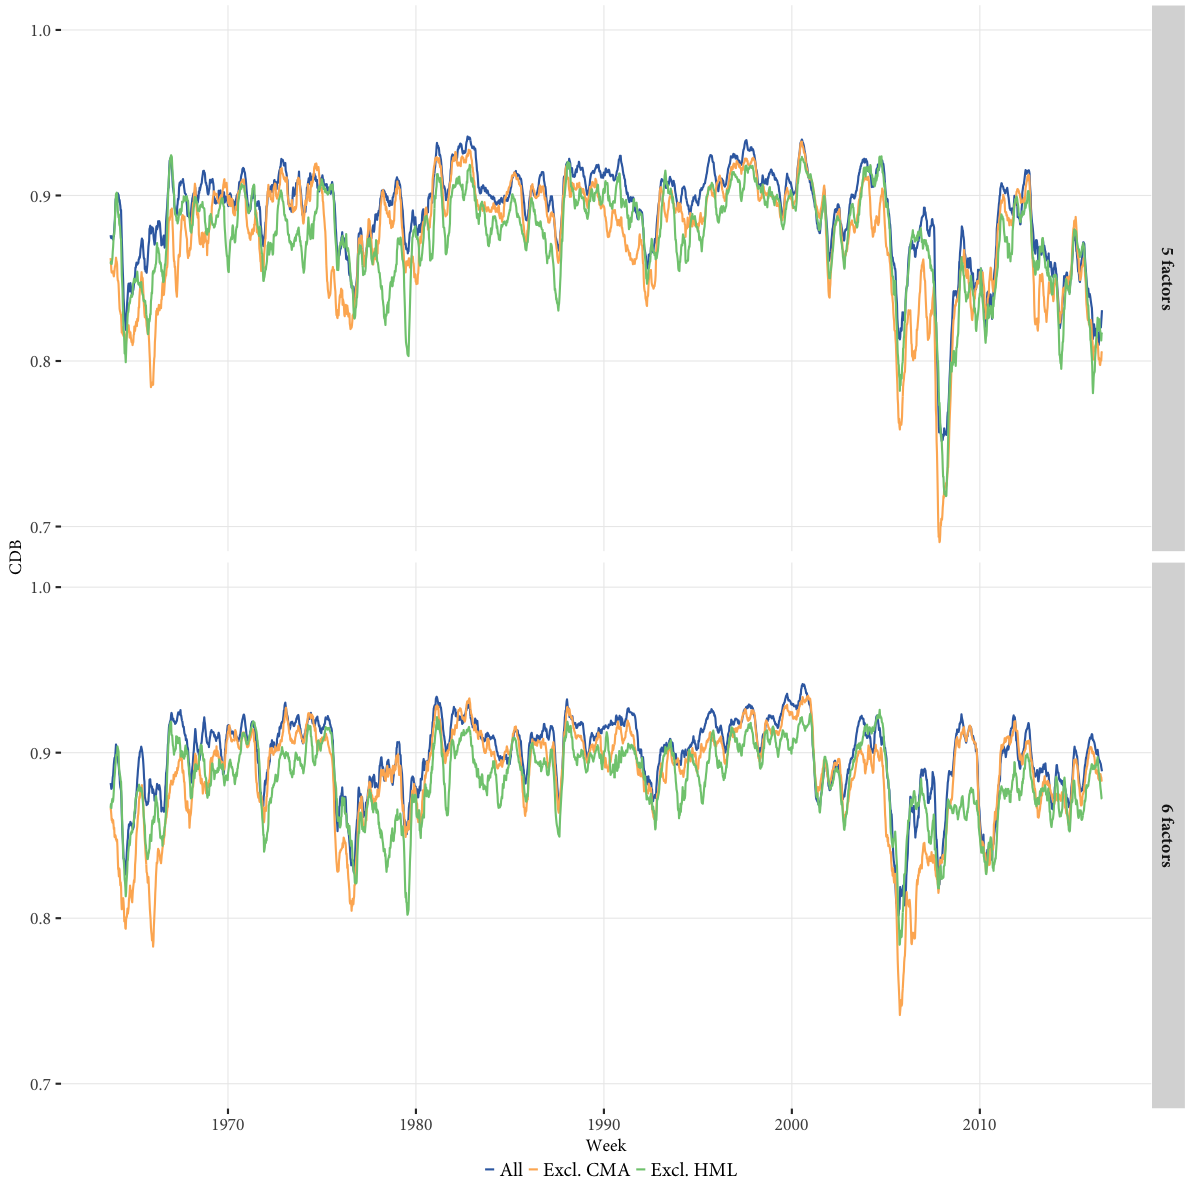
\includegraphics[scale = 1]{graphics/cdb_5F_6F.png}
\end{figure}

% CDB is very high; factor strategies are good diversifiers
First, we note that regardless of whether momentum is included or not, factor strategies appear to offer high levels of diversification. In absolute terms, all strategies sit close to or above $0.90$ for the majority of the studied time period. [Why is this high. We need to relate it to something] The differences between strategies are small with a high degree of overlap; given the uncertainty in estimates, the small differences must be interpreted conservatively.

% Dips
Second, there are notable dips in the diversification benefit measure. The dips represent times when diversification is relatively hard to come by, and roughly coincide in the five- and six-factor models.

% HML is a better diversifier on average
% CMA better when diversification is hard to come by
Third, a complicated picture appears when comparing the diversification benefits offered by substituting HML for CMA, and vice versa. Looking at the six factor portfolio, the strategy where HML is excluded has a lower level of diversification benefit on most weeks compared to where CMA is excluded. This pattern appears reversed at critical times, however: When the full six factor CDB is low -- before 1965, around 1978, 2007 and 2011 -- the maximum diversification benefit of an HML strategy is in all cases except 2011 below that of the CMA strategy. HML thus appears to be the better diversifier in normal times, however, when diversification is hard to come by, CMA outperforms it. Excluding Momentum, the status of HML as a superior diversifier in normal times is much less clear; while its underperformance is even more noticeable when diversification potential is lower.

\autoref{tab:cdb_table} displays CDB summary statistics and the results of paired t-tests of the differences between strategies. This table tells the same story as the graph. In a five-factor setting, there is no significant difference in the expected diversification benefit from swapping CMA for HML, however, HML is a significantly better diversifier in a six-factor setting. Although the difference is significant, it is small and does not account for the uncertainty in the estimation of the model that is the basis for the portfolio return distribution.

%!TEX root = ../../main.tex

\begin{table}
  \centering
  \footnotesize
  \renewcommand{\arraystretch}{1.2}
  
  \caption{Conditional diversification benefit (CDB)\\ \quad \\
  Based on symmetric dynamic copula model, full sample (1963--2016). \emph{Difference} shows the average pair-wise difference in CDB between the column's and row's strategy, respectively, with t-test standard errors and significance levels (the first pair is thus the difference in pair-wise CDB between a five-factor strategy with and without CMA)}

  \begin{tabularx}{\textwidth}{@{} l X dddd X dd @{}}
    \toprule
    &&
      \multicolumn{4}{c}{CDB} && 
      \multicolumn{2}{c}{Difference} \\
    \cmidrule{3-6} \cmidrule{8-9}
    &&
      \multicolumn{1}{c}{Mean} &
      \multicolumn{1}{c}{SD} &
      \multicolumn{1}{c}{Min} &
      \multicolumn{1}{c}{Max} &&
      \multicolumn{1}{c}{All} &
      \multicolumn{1}{c}{Excl. CMA} \\
    \midrule
    \textbf{Five Factors} \\
    \emph{All}       && 88.937 & 3.410 & 61.469 & 95.135 &&   &                        \\
                     &&        &       &        &        &&   &                        \\
    \emph{excl. CMA} && 87.439 & 4.221 & 61.346 & 95.105 &&   1.497^{***} &             \\
                     &&        &       &        &        &&  (0.053)      &             \\
    \emph{excl. HML} && 87.448 & 3.731 & 61.722 & 94.274 &&   1.489^{***} & -0.009      \\
                     &&        &       &        &        &&  (0.050)      & (0.065)     \\
    \midrule
    \textbf{Six Factors} \\
    \emph{All}       && 89.783 & 2.898 & 72.850 & 95.043 &&   &                       \\
                     &&        &       &        &        &&   &                       \\
    \emph{excl. CMA} && 88.602 & 3.657 & 69.143 & 95.160 &&  1.181^{***} &             \\
                     &&        &       &        &        && (0.050)      &             \\
    \emph{excl. HML} && 88.259 & 3.053 & 71.987 & 94.447 &&  1.524^{***} &  0.343^{***}  \\
                     &&        &       &        &        && (0.049)      & (0.060)     \\
    \bottomrule
  \end{tabularx}

  \label{tab:cdb_table}
\end{table}


% What periods does low CDB correspond to?
% Story related to threshold correlations and patterns seen Mkt-HML

% No obvious corresponde with the market's performance. This does not appear
% to be related to the tail dependency so mcuh...

% subsection conditional_diversification_benefit (end)
